\chapter{One Sample Confidence Intervals on a Mean When the Population Variance is Known}
\section{Key Concepts and Definitions}

\begin{definitionbox}{Key Terms}
\textbf{Population:} A group of interest (typically large). \\
\vspace{0.2em}

\textbf{Sample:} A subset of a population. \\

\textbf{Parameter (of population):} A numerical characteristic of a population. These are usually \textcolor{blue}{unknown} in real-life settings. \\
\hspace*{1em} $\mu$: population mean \\
\hspace*{1em} $\sigma^2$: population variance \\
\hspace*{1em} $\sigma$: population standard deviation \\
\textcolor{blue}{Note: Different from a parameter of a distribution.} \\

\textbf{Statistic (of sample):} A numerical characteristic of a sample, which is calculated and known (i.e., a function of the data). \\
\hspace*{1em} $\bar{x}$: sample mean \\
\hspace*{1em} $s^2$: sample variance \\
\hspace*{1em} $s$: sample standard deviation\\
\vspace{0.2em}

\textbf{Statistical Inference:} Use statistics (known) to make conclusions on parameters (unknown) and quantify the degree of certainty of statements made.

\end{definitionbox}
\noindent
The sample mean, $\bar{x} = \frac{1}{n} \sum_{i=1}^{n} x_i$, is a number we use to estimate the population mean, $\mu$. This is called a \textbf{point estimate}. % one value, single best estimate of a parameter

\vspace{1em}

But, we know it’s not equal to $\mu$. Then, we’d rather estimate the population mean using an \textbf{interval estimate} that gives a \textit{range of real numbers} that we hope contains the population mean, $\mu$.
\vspace{2em}
\textcolor{orange!80!black}{\section*{Examples}}

\begin{itemize}
    \item $\bar{x}$ is a point estimate of $\mu$
    \item $s^2$ is a point estimate of $\sigma^2$
    \item $s$ is a point estimate of $\sigma$
\end{itemize}

\vspace{0.5em}
\textcolor{blue}{\textit{(All calculated with data from a sample)}}

\vspace{1.5em}

Due to the nature of randomness and calculating based on a subset, statistics are not guaranteed to be exactly equal to parameters.

\vspace{1em}

Therefore, we create \underline{intervals} around statistics which we believe capture the parameter.

\vspace{2em}

\noindent
\textbf{Confidence Interval:} A range of values we believe captures a parameter with a certain level of confidence.

\vspace{1em}

\begin{center}
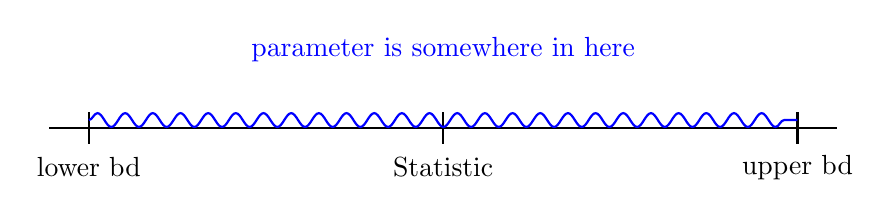
\begin{tikzpicture}
    \draw[thick] (-5,0) -- (5,0);
    \draw[thick] (-4.5,0.2) -- (-4.5,-0.2); % lower bd
    \draw[thick] (0,0.2) -- (0,-0.2);       % statistic
    \draw[thick] (4.5,0.2) -- (4.5,-0.2);   % upper bd
    \node at (-4.5,-0.5) {lower bd};
    \node at (0,-0.5) {Statistic};
    \node at (4.5,-0.5) {upper bd};
    \node[blue] at (0,1) {parameter is somewhere in here};
    \draw[blue, thick, decorate, decoration={snake}] (-4.5,0.1) -- (4.5,0.1);
\end{tikzpicture}
\end{center}

\vspace{2em}

\noindent
\textbf{Skeleton (general form):}
\[
\text{Estimator (statistic)} \pm \left( \text{value from a reference distribution} \times \text{standard error of estimate} \right)
\]

\vspace{0.5em}
\textcolor{blue}{\textit{Z or t} \hspace{1em} \textit{Standard error = std. dev. of sampling distribution}}

\vspace{1em}
The exact form depends on the parameter of interest and the information available.

\vspace{2em}

\textbf{Interpretation of CI’s:}

Suppose we construct a $C\%$ confidence interval.

\vspace{0.5em}
\textbf{Intuitive Interpretation:} We are $C\%$ confident the target parameter is inside the CI constructed.

\vspace{0.5em}
\textbf{Formal Definition:} In repeated sampling, approximately $C\%$ out of all the $C\%$ CI’s constructed captures the parameter.

\vspace{1em}
(See Slide 11)

\vspace{2em}

\begin{center}
% \includegraphics[width=0.85\textwidth]{ci_visual.png}
\begin{center}
\fbox{\parbox{0.8\textwidth}{
\centering
[Insert visual showing 95\% confidence intervals for $\mu$ -- see slide image with intervals]}
}
\end{center}

\end{center}

\vspace{0.5em}
Approximately 95\% of the 1000 intervals (i.e., approx. 950) capture $\mu$.
